\documentclass{article}
\usepackage{amsmath}
\usepackage{amssymb}
\usepackage{color}
\usepackage[utf8]{inputenc}
\usepackage{tikz}
\usetikzlibrary{positioning}
\usetikzlibrary{decorations,arrows,shapes}
\usepackage{tikz-cd}

\begin{document}

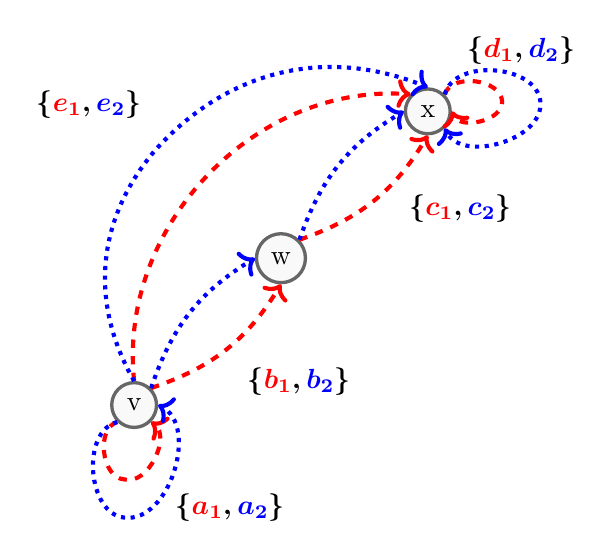
\begin{tikzpicture}[roundnode/.style={circle, draw=black!60, fill=gray!5, very thick, minimum size=3mm}]
        %Nodes
        \node[roundnode]     (w)                             {w};
        \node[roundnode]        (x)       [above right=2 of w] {x};
        \node[roundnode]      (v)       [below left= 2 of w] {v};
        \node[]             (xl1)        [right = .5 of x] {};
        \node[]             (xl2)        [right = 1 of x] {};
        \node[]             (vl1)        [below= .5 of v]    {};
        \node[]             (vl2)        [below= 1 of v]    {};
        \node[]             (u)         [above left = 1.6 of w] {};
        
        %Lines
        \draw[->,line width = 1.5, draw = red, dashed] (w.north east) to[bend right = 20]  (x.south);
        \draw[->,line width = 1.5, draw = red, dashed] (v.north east) to[bend right = 20] (w.south);
        \draw[->,line width = 1.5, draw = blue, dotted] (w.north east) to[bend left = 20]  (x.west);
        \draw[->,line width = 1.5, draw = blue, dotted] (v.north east) to[bend left = 20] (w.west);
        
        \draw[->, line width = 1.5, draw = red, dashed, dashed] (v.south west) to[in=90, bend right = 80] (vl1) to[out=270, in=10, bend right = 80] (v.south east);
        \draw[->, line width = 1.5, draw = blue, dotted] (v.south west) to[in=90, bend right = 80] (vl2) to[out=270, in=10, bend right = 80] (v.east);
        
        \draw[->, line width = 1.5, draw = red, dashed, dashed] (x.north east) to[in=90, bend left = 80] (xl1) to[out=270, in=10, bend left = 80] (x.east);
        \draw[->, line width = 1.5, draw = blue, dotted] (x.north east) to[in=90, bend left = 80] (xl2) to[out=270, bend left = 80] (x.south east);
        
        \draw[->, line width = 1.5, draw = red, dashed, dashed] (v.north) to[bend left= 50] (x.north west);
        \draw[->, line width = 1.5, draw = blue, dotted] (v.north) to[bend left= 35] (u) to[bend left= 35] (x.north);
        
        %Labels
        \node[]     (a)     [below right = 1 and .1  of v.east]  {$\boldsymbol{\{{\color{red}a_1},{\color{blue}a_2}\}}$};
        \node[]     (b)     [above right = 1 and .1  of a.north]  {$\boldsymbol{\{{\color{red}b_1},{\color{blue}b_2}\}}$};
        \node[]     (c)     [above right = 1.6 and .5  of b]  {$\boldsymbol{\{{\color{red}c_1},{\color{blue}c_2}\}}$};
        \node[]     (d)     [above = 1.7  of c.east]  {$\boldsymbol{\{{\color{red}d_1},{\color{blue}d_2}\}}$};
        \node[]     (e)     [above left = 2 of w.north west]    {$\boldsymbol{\{{\color{red}e_1},{\color{blue}e_2}\}}$};
        
        
        
        \end{tikzpicture}

\end{document}